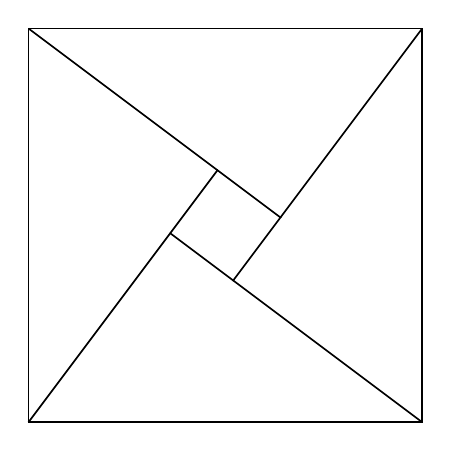
\begin{tikzpicture}[x=1cm,y=1cm,font=\normalsize,
 geometry edge/.style={solid,line width=.6pt},
 geometry mark/.style={solid,line width=.6pt},
 geometry label/.style={font=\normalsize,inner sep=2pt}]
\coordinate (Q0) at (0,0);
\coordinate (Q1) at (5,0);
\coordinate (Q2) at (5,5);
\coordinate (Q3) at (0,5);
\coordinate (S0) at (1.8,2.4);
\coordinate (S1) at (2.6,1.8);
\coordinate (S2) at (3.2,2.6);
\coordinate (S3) at (2.4,3.2);
\draw[geometry edge] (Q0)--(Q1)--(Q2)--(Q3)--cycle;
\draw[geometry edge] (Q0)--(S0);
\draw[geometry edge] (Q1)--(S1);
\draw[geometry edge] (Q2)--(S2);
\draw[geometry edge] (Q3)--(S3);
\draw[geometry edge] (S0)--(S1)--(S2)--(S3)--cycle;
\end{tikzpicture}
